
Im Rahmen dieser Arbeit wurden verschiedene Technologien und Prinzipien eingesetzt. Auf diese soll in den folgenden Unterkapiteln eingegangen werden, damit eine theoretische Grundlage vorhanden ist. 

\subsection{\ac{UDP}}
\label{sec:UDP-1}

\ac{UDP} steht für ``User-Datagram-Protocol'' und ist ein verbindungsloses Transportprotokoll. Im \ac{OSI}-7-Schichten Modell arbeitet es auf der Transportebene und ist für die Zustellung von Netzwerkpaketen von einem Sender zu einem Empfänger zuständig. Im Vergleich zum Transportprotokoll \ac{TCP}, welches verbindungsorientiert arbeitet, ist es wesentlich einfacher zu verarbeiten, da beispielsweise der Header bei den einzelnen Datenpaketen wesentlich kleiner ist. Allgemein ist es sehr minimal gehalten und dadurch sehr einfach zu implementieren und für sehr einfache Anwendungszwecke geeignet. Allerdings ist auch zu erwähnen, dass es keine Empfangsbestätigung gibt und die Daten nach dem Absenden nicht weiter kontrolliert werden. Somit können die Daten auch im Netzwerk verloren gehen und es wird nicht bemerkt. \\
Der einfache Header des \ac{UDP} Protokolls besteht nur aus vier Attributen. Diese jeweils 16 Bit großen Felder enthalten den Quellport, den Zielport, die Checksumme zur Überprüfung des Inhalts und die Länge des gesamten Pakets. Insgesamt ist der Header somit 8 Byte groß. (vgl. \cite{ElektronikKompendium.}\cite{.}\cite{.23.02.2016})
 

\subsection{\ac{TCP}}
\label{sec:TCP-1}

\ac{TCP} ist ein verbindungsorientiertes Protokoll, dass im \ac{OSI}-7-Schichten Modell auf der vierten Ebene (Transport) einzuordnen ist. Im sogenannten \ac{TCP}/\ac{IP} Protokollstapel ist es in der dritten von vier Schichten zu finden. Bei einer Übertragung von Daten über \ac{TCP} übergibt die genutzte Anwendung den Datenstrom an das Protokoll und empfängt ihn auch wieder von dort. Für die Übertragung ist dementsprechend \ac{TCP} zuständig. 
Die Hauptaufgaben des Protokolls sind daher die Aufteilung und die Zusammensetzung der Daten von entsprechend vielen Paketen (Segmentierung), das Management der Verbindung und ein entsprechendes Fehlerhandling, welches das korrekte Empfangen von Paketen überwacht. Das Fehlerhandling nutzt eine positive Bestätigung aller Pakete. Dies bedeutet, dass nur nicht vorhandene Pakete erneut angefragt werden, ansonsten davon ausgegangen wird, dass die Daten beim Empfänger angekommen sind. Diese Technologie sorgt dafür, dass die Daten auf jeden Fall ankommen, sofern die Verbindung nicht gestört wird (vgl. \cite{.c}\cite{.22.11.2016}).

Der Header eines \ac{TCP} Pakets besteht aus 20 Bytes, jedoch kann dieser auch noch erweitert werden, sodass noch einige zusätzliche Bytes in den Header geschrieben werden. Zu den zwingend notwendigen Daten gehört unter anderem der Port auf dem das Paket empfangen wird und der Port über den das Paket gesendet wird. Zudem wird die Nummer im aktuellen Paketstrom benötigt. Zudem wird eine Prüfsumme und Quittierungsnummer mitgegeben, welche zur Kontrolle und Bestätigung genutzt werden (vgl \cite{.c}).


\subsection{Webserver: Nginx}
\label{sec:WebserverNginx-1} 

Nginx bestitzt einen Marktanteil von ca. 20 Prozent aller Webserver und ist somit auf Rang 2 der Webserver für aktive Webseiten hinter Apache und vor Microsoft und Google\cite{.k}. In dieser Studienarbeit haben wir uns für nginx entschieden, da ein hoher Wert auf eine flexible Konfiguration und schnelle Serverantworten gelegt wird. Folgend werden die Hauptfeatures von Nginx genauer beschrieben.

\subsubsection{Allgemein}
\label{sec:NginxAllgemein}
Nginx ist ein HTTP und Reverse-Proxy Server, ein Mail-Proxy Server und ein allgemeiner TCP/UDP Proxy-Server. Somit hat Nginx eine hohe Nutzungsbreite.

\subsubsection{Features}
\label{sec:NginxFeatures}
Die von Nginx unterstützten Features werden im Folgenden gegliedert nach den jeweiligen Einsatzgebeiten vorgestellt.\cite{.14.03.2017}


\subsubsection{Basic HTTP}
\label{sec:NginxBasicHTTP}
Nginx unterstützt die Bereitstellung von statischen Dateien. Durch die modulare Architektur ist Nginx für viele Zwecke einsetzbar und bleibt dabei übersichtlich. HTTP/2 wird unterstützt, was die Übertragung beschleunigt und optimiert. Das Rewrite Modul ermöglicht die Änderungen von URIs anhand von regulären Ausdrücken. Dies trägt auch zur Suchmaschinenoptimierung bei und ermöglicht das Erstellen von lesbaren URIs. Die Zugriffskontrolle kann anhand von IP-Adressen oder Passwörtern erfolgen. Anhand der IP-Adresse können zudem Informationen zu Geolocation gewonnen werden. SSL und TLS SNI wird natürlich auch unterstützt.

\subsubsection{Mail Proxy-Server}
\label{sec:NginxMail Proxy-Server}
Die Authentifizierung kann über einen externen HTTP Server durchgeführt werden, welcher dann nach erfolgreicher Authentifizierung zu einem internen SMTP-Server weiterleitet. Somit muss man sich nicht direkt am Mail-Server authentifizieren. Zudem wird SSL, STARTTLS und STLS unterstützt.

\subsubsection{TCP/UDP Proxy-Server}
\label{sec:NginxTCP/UDP Proxy-Server}
Allgemeine Proxy-Features von TCP und UDP sind vorhanden. Des Weiteren wird SSL und TLS SNI auch für TCP unterstützt.
Um vor Überlastungen zu schützen können Verbindungen, die von derselben Adresse kommen begrenzt werden. Zugriffskontrolle geschieht anhand der Benutzeradresse. Es werden zudem auch Features unterstützt, die den Lastausgleich und die Fehlertoleranz verbessern.


\subsubsection{Architektur und Skalierbarkeit}
\label{sec:NginxArchitektur und Skalierbarkeit}
Nginx ist so aufgebaut, dass es einen Master und mehrere Worker-Prozesse gibt. Die Worker brauchen dabei keinerlei spezielle Berechtigungen, so muss nur dem Master entsprechende Berechtigungen gewährt werden. Des Weiteren ist eine flexible Konfiguration möglich. Die Nginx Konfiguration für diese Studienarbeit befindet sich im Anhang unter Abschnitt \ref {sec:NginxKonfiguration}.

 
\subsection{Arduino}
\label{sec:Arduino-1} 

Die Bezeichnung Arduino steht für eine Technologie, die sowohl aus einer Hardwarekomponente als auch aus einer Softwarekomponente besteht. Zudem gibt es zwei Unternehmen, die in ihrem Namen den Begriff Arduino tragen und in Zusammenhang mit der Technologie stehen. Zum einem gibt es die Arduino LLC, die die Gruppe der Gründer der Plattform bezeichnet. Des Weiteren gibt es die Arduino S.r.l., das die Firma bezeichnet, die anfangs allein die Arduinoboards produzierte und dann auch verkaufte. Die Arduinoplattform wurde ursprünglich entwickelt, um Anfängern den Einstieg in die Mikrokontrollerprogrammierung zu vereinfachen. 

Grundsätzlich besteht die sogenannte Arduinoplattform aber sowohl aus der Hardware als auch der Software. Die Hardware umfasst mittlerweile verschiedene Mikrokontroller beziehungsweise Einplatinencomputer, welche für verschiedene Anwendungszwecke genutzt werden können. Die entsprechende Nutzung wird mithilfe der richtigen Programmierung erreicht. Dafür kann der Softwareteil der Lösung genutzt werden, welches aus einer \ac{IDE}  besteht und das Schreiben von Programmen vereinfacht. Zudem wird über diese \ac{IDE} auch die Kommunikation mit dem Mikrokontroller realisiert. Diese Entwicklungsumgebung eignet sich für diverse Mikrokontroller, sofern entsprechende Treiber verfügbar sind, können auch Boards genutzt werden, die nicht direkt mit Arduino zusammenhängen. Zudem kann in verschiedenen Programmiersprachen entwickelt werden, beispielsweise C oder C++. (vgl. \cite{.h,.f,.e,.i,.g,online.})
Die komplette Plattform ist open source, auch wenn die Hardware natürlich erworben werden muss. 



\subsection{Python}
\label{src:Python-1}

Python ist eine objektorientierte Programmiersprache und wurde 1991 in der ersten Version von Guido van Rossum veröffentlicht (vgl. \cite{.05.03.2017}). Zu den technischen Merkmalen gehört unter anderem die Unterstützung von Paketen beziehungsweise Bibliotheken, die die entsprechend benötigten Funktionen laden, sofern sie in das Projekt eingebunden werden. 

Außerdem ist eines der Merkmale die Einrückung. Python nutzt nicht, im Gegensatz zu anderen Programmiersprachen, bestimmte Klammern oder andere Symbole um den Code zu strukturieren, sondern verwendet stattdessen die Einrückung von den entsprechenden Zeilen Code. Das bedeutet, dass zum Beispiel nach einem Methodenkopf keine geschweifte Klammer oder ähnliches verwendet wird, sondern die nächste Zeile wird um beispielsweise vier Leerzeichen eingerückt. Das Methodenende wird dadurch definiert, dass ein anderer Codeabschnitt wieder auf der gleichen Einrückungsstufe steht, wie der Methodenkopf (vgl. \cite{.19.08.2013}\cite{.10.03.2017b}). 
Zudem ist Python eine dynamische Programmiersprache und es ist möglich Python als Skriptsprache zu verwenden und Skripte zu schreiben, die mithilfe des Interpreters ausgeführt werden. Durch die Möglichkeit Python auch auf Linux zu verwenden, können diese Skripte auch entsprechend unter Linux verwendet werden.

Python kann für verschiedene Anwendungszwecke genutzt werden, es gibt zum Beispiel verschiedene Möglichkeiten der Stringverarbeitung, die Möglichkeit mit verschiedenen Internetprotokollen zu arbeiten, beispielsweise \ac{HTTP}, \ac{FTP} oder \ac{SMTP} aber auch auf Interfaces des Betriebssystems zuzugreifen, um beispielsweise mit Sockets (z.B. \ac{TCP}/\ac{IP} Sockets) zu arbeiten. Neben diesen Funktionen, die durch die Standardbibliotheken abgedeckt werden, gibt es auch noch weitere Pakete, die weitere Bibliotheken mit Funktionen hinzufügen. So gibt es zum Beispiel die Möglichkeit das Paket BeautifulSoup oder Requests hinzuzufügen. Letzteres bietet zum Beispiel viele Möglichkeiten mit dem \ac{HTTP} Protokoll zu arbeiten (vgl \cite{.m}\cite{.l}\cite{.05.03.2017}). 



\subsection{WLAN-Chipsatz}
\label{sec:WLAN-CHipsatz-1} 

\subsection{MySQL}
\label{sec:MySQL-1}
 
\subsection{Frontendtechnologien}
\label{sec:Frontendtechnologien-1}

Um eine dynamische und nutzerfreundliche Oberfläche zu schaffen wurden Frameworks benutzt. 
Für die Gestaltung der einzelnen Komponenten wurde Bootstrap verwendet, welches für alle wichtigen Komponenten bereits vorgefertigte Styles enthält.
Dies beschleunigt den Prozess der Gestaltung der Oberfläche enorm, da nicht jede verwendete Komponente manuell anhand von \ac{CSS} gestaltet werden muss. 
Die verwendete Bootstrap Version ist Version 3.

Bootstrap ermöglicht es ohne großen Aufwand responsive Webseiten zu gestalten. 
Dabei soll während der Entwicklung auf das mobile-first Prinzip Wert gelegt werden. 
Dieses Prinzip besagt, dass zuerst die Seite für mobile Endgeräte optimiert wird und anschließend erst auf größere Monitore beziehungsweise Auflösungen geachtet werden soll. 
Weltweit liegt der Anteil aller Website-Aufrufe von mobilen Endgeräten bei fast 50\% (vgl. \cite{.stat-mobile}). 

Für die Dynamik sorgt das JavaScript-Framework Vue. Mit Vue vergleichbare Frameworks sind React und Angular. Vue wird verwendet, da es eine große Community hat, eine gute Dokumentation vorweist, sowie eines der besten Frameworks performancetechnisch ist (vgl. \cite{.vue-react-angular}).
Frontend Frameworks, wie auch Vue, bieten die Funktionalität Komponenten zu erstellen und diese beliebig zu verwenden. 
Des Weiteren erhöhen sie, vorausgesetzt sie werden richtig eingesetzt, die Nutzererfahrung, da nicht bei jeder Aktion die komplette Seite neu geladen werden muss.

Folgend wird etwas genauer auf das Vue-Framework eingegangen. 
Komponenten sind das Herzstück von Vue. Sie besitzen jeweils genau ein Template, welches in \ac{HTML} definiert ist. 
Des Weiteren haben Komponenten Daten, die durch data-binding automatisiert geändert werden. 
Beispielsweise kann man eine Variable an ein Input-Element binden und wenn dieses einen anderen Wert annimmt wird auch automatisch die Variable angepasst. 
Daten können dabei direkt bei der Initialisierung der Komponente oder zu einem späteren Zeitpunkt geladen werden.
Dadurch wird die initiale Ladezeit der Seite deutlich verringert, da die Daten asynchron geladen werden.

 
 \newpage
 
\subsection{\ac{REST}}        
\label{sec:REST-1}  
\subsubsection{\ac{REST} Allgemein}
\label{sec:RESTAllgemein}

Im Folgenden soll die Technologie \ac{REST} vorgestellt werden.
Zunächst wird \ac{REST} etwas genauer anhand von Beispielen erläutert.
Anschließend werden die Vor- und Nachteile dargestellt, sowie die Kernpunkte erläutert.

\subsubsection{\ac{REST} Beispiel}
\label{sec:RESTBeispiel}

Um Daten von einer \ac{REST}-Schnittstelle zu bekommen, werden die \ac{HTTP}-Methoden in Verbindung mit einer entsprechenden \ac{URI} verwendet. Im Folgenden wird dies anhand einiger Beispiele gezeigt:

GET /resources/
Liefert eine Liste aller Ressourcen.

GET /resources/4
Liefert die Ressource mit ID = 4.

POST /resources/
Legt eine neue Ressource an.

PUT /resources/4
Aktualisiert die Ressource mit ID = 4.

DELETE /resources/4
Löscht die Ressource mit ID = 4.

Einen tieferen Einblick, wann und wie die Methoden genutzt werden, wird in Abschnitt \ref{sec:RESTHTTP} gegeben.

\subsubsection{Ressourcen}
\label{sec:RESTRessourcen}

Im Folgenden werden Datensätze als Ressourcen bezeichnet. Dabei kann man die Ressourcen weiter unterteilen:

–	Primärressourcen: Unter Primärressourcen fallen komplette, vollständige Ressourcen

–	Subressourcen: Subressourcen sind Teile von Primärressourcen

–	Listen: Eine Liste umfasst eine Menge von Ressourcen

–	Filter: Anwendung von Filterkriterien auf Listen

–	Paginierung: begrenzte Datenmenge

–	Projektionen: Teil der Informationen einer Primärressource

–	Aggregationen: Zusammenfassung mehrerer Ressourcen

\subsubsection{Merkmale}
\label{sec:RESTMerkmale}

Die Kommunikation erfolgt auf Abruf. Der Client ist aktiv und fordert vom passiven Server eine Repräsentation an, bzw. modifiziert eine Ressource. Ressourcen, die Objekte der Anwendung, besitzen eine ihnen zugeordnete \ac{URI}, mit der sie adressiert werden können. Die Repräsentation einer Ressource kann als Dokument vom Client angefordert werden. Repräsentationen können auf weitere Ressourcen verweisen, die ihrerseits wieder Repräsentationen liefern, die wiederum auf Ressourcen verweisen können. Der Server verfolgt keinen Clientstatus. Jede Anfrage an den Server muss alle Informationen beinhalten, die zum Interpretieren der Anfrage notwendig sind. Caches werden unterstützt. Der Server kann seine Antwort als cache-fähig oder nicht cache-fähig kennzeichnen.

Repräsentationen:

Um die Ressourcen darzustellen, werden in REST mehrere Repräsentationen der Ressourcen genutzt. Dies entsteht aus der Intention heraus, dass aufgrund der unterschiedlichen Repräsentationen unterschiedliche Anforderungen der Clients bedient werden können. So kann zum Beispiel die \ac{HTML} Repräsentation für einen Webbrowser genutzt werden, während eine \ac{JSON} Repräsentation für eine Clientapplikation genutzt wird.

\subsubsection{HTTP}
\label{sec:RESTHTTP}


Um auf eine Ressource zuzugreifen wird das \ac{HTTP}-Protokoll verwendet. Je nachdem, welche Verwendung die Ressourcen finden, werden geeignete \ac{HTTP}-Methoden verwendet. Die häufigsten Verwendeten Methoden sind dabei GET, POST, PUT und DELETE. Per GET werden Daten geladen; POST hat mehrere Einsatzgebiete. Häufig wird dadurch eine neuer Datensatz angelegt, oder mehrere Datensätzen aktualisiert. PUT aktualisiert einen bestimmten Datensatz und DELETE löscht einen Datensatz. Dabei müssen sinnvolle Statuscodes zurückgegeben werden. Zusätzlich gibt es noch die Methoden PATCH, HEAD und OPTIONS. Auf diese wird jedoch nicht weiter eingegangen, da diese eine vergleichsweise geringe Bedeutung bei einer REST-Schnittstelle haben. Bei der Implementierung ist unbedingt zu beachten die Methoden idempotent zu gestalten, d.h. Ein mehrmaliges Aufrufen derselben Methode wirkt sich nicht anders aus, als ein einmaliger Aufruf. Einzige Ausnahme dabei ist die POST-Methode. Das Prinzip von \ac{REST} ist, Ressourcen von einem Zustand in den nächsten Zustand zu überführen.

\subsubsection{Statuscodes}
\label{sec:RESTStatuscodes}

Folgende Tabelle zeigt die allgemeine Bedeutung der unterschiedlichen Statuscodes

\begin{table}[!h]
	\begin{tabular}{ | l | l | }
		\hline
		Statuscode & Bedeutung \\ \hline
		1xx & Informationen \\ \hline
		2xx & Erfolgreiche Operationen \\ \hline
		3xx & Umleitung \\ \hline
		4xx & Client-Fehler \\ \hline
		5xx & Server-Fehler \\ \hline
	\end{tabular}
	\caption{Statuscodes}
\end{table}


\subsubsection{URI-Design}
\label{sec:RESTURI-Design}

Eine \ac{URL} lokalisiert eine Ressource, wobei eine \ac{URI} sie identifiziert. Lokalisierung kann dabei auch zur Identifizierung führen.
Eine \ac{URL} ist also immer eine \ac{URI}. Im Umkehrschluss kann eine \ac{URI} eine \ac{URL} sein, muss es
aber nicht.

Möchte man \ac{REST} in einem Satz definieren, dann ergibt sich: „Eine eigene URI für jedes Informationselement.“ (vgl. \cite{.j}\cite{Tilkov.2015b})

An diesem Satz sollte man sich auch beim \ac{URI}-Design halten. Ressourcen können so durch
ihre \ac{URI} eindeutig identifiziert werden. Dabei sollen diese so konstruiert werden, dass man
bereits aus der \ac{URI} alleine lesen kann, was für eine Ressource dahinter steckt. Eine \ac{URI} zeigt
auf eine Ressource, aber diese kann über mehrere \ac{URI}s angesprochen werden.
Die verschiedenen Ressourcenarten können auf folgende \ac{URI}-Strukturen abgebildet werden (vgl. Kapitel \ref{sec:RESTRessourcen}): 

–	Liste: /resources/:	Man bekommt mehrere Ressourcen gleicher Art

–	Primärressource: /resources/1:	Man bekommt genau eine unabhängige Ressource

–	Sekundärressource: /resources/subresources/1:	Man bekommt genau eine von einer anderen Ressource abhängige Ressource

–	Filter: /resources?name=a oder /resources/name=a : Man bekommt mehrere Ressourcen gleicher Art, die mit bestimmten Parametern gefiltert werden.

\subsubsection{HATEOAS}
\label{sec:RESTHATEOAS}

HATEOAS ist ein wichtiges Prinzip, welches von vielen selbsternannten \ac{REST}-Schnittstellen
nicht implementiert wird. Dieses Akronym beschreibt, dass die Schnittstelle über Hypertext
beziehungsweise Hypermedia angetrieben wird. Genauer gesagt, sollen durch den Aufruf
der Haupt-URI alle Funktionalitäten als Hyperlinks unter Angabe der jeweiligen Beziehung
zugreifbar sein. Die Schnittstelle dokumentiert sich sozusagen selbst.
In seiner im Jahre 2000 verfassten Dissertation “Architectural Styles and the Design of
Network-based Software Architectures”, definiert Roy Fielding die \ac{REST}-Architektur. Dabei
geht er unter anderem auf Ressourcen und \ac{HTTP} ein. Als wichtigen Punkt sieht Fielding
jedoch auch die Verwendung von Hypermedia und die Verlinkung zwischen verwandten Ressourcen.
In 2008 verdeutlicht Fielding anhand eines Blogeintrags seinen Standpunkt zu RESTful API’s...
“If the engine of application state (and hence the API) is not being driven by hypertext, then
it cannot be RESTful and cannot be a REST API. Period. Is there some broken manual
somewhere that needs to be fixed?” – \cite{.19.03.2017}

Damit will er sagen, dass Schnittstellen, welche nicht über Hypertext gesteuert werden, auch
keine \ac{REST}-Schnittstellen sind, sondern ganz normale RPC-Schnittstellen.
Um dieses Prinzip zu verdeutlichen wird anhand Abbildung 3 das Richardson Maturity Model
veranschaulicht.
 
\begin{figure}[!htb]
	\centering
	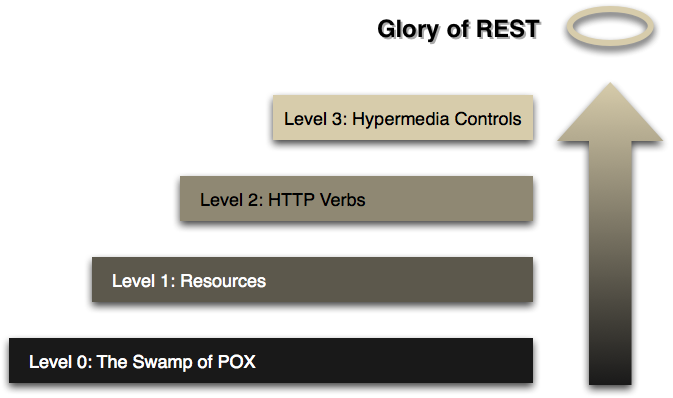
\includegraphics[scale=0.5]{hateoas.png}
	\caption[Richardson Maturity Model]{Richardson Maturity Model,\\ Quelle: https://martinfowler.com/articles/images/richardsonMaturityModel/ overview.png}
\end{figure}
 


Das Richardson Maturity Model unterteilt die \ac{REST}-Architektur in vier Stufen. Eine echte
\ac{REST}-Schnittstelle implementiert dabei alle vier Stufen. Doch gerade die letzte Stufe wird oft
nicht implementiert, da sie eine gewisse Komplexität birgt.

LEVEL 0 sagt lediglich aus, dass \ac{HTTP} als Transportprotokoll für RPC-Aufrufe genutzt wird.
Die Kommunikation findet über eine einzige \ac{URI} statt.

LEVEL 1 sagt aus, dass jede Ressource eine eigene \ac{URI} hat.

In LEVEL 2 werden die bereits Vorgestellten \ac{HTTP}-Methoden verwendet.

In der letzten Stufe, LEVEL 3, kristallisieren sich die Unterschiede zwischen richtigen \ac{REST}-
Services und solchen, die es gerne sein wollen. Durch den Einsatz von Hypermedia sollen alle
Ressourcen miteinander verknüpft werden. Dabei soll beim Aufruf der Haupt-\ac{URI} alle
möglichen Aufrufe zurückgegeben werden. Folgende Tabelle soll die Vor- und Nachteile von
HATEOAS verdeutlichen.
\newline

\begin{table}[H]
	\begin{tabular}{ | p{7cm} | p{7cm} | }	
		\hline	
		Vorteile & Nachteile \\  \hline	
		Entkopplung von Client und Server, da sich der Client nicht anpassen muss,
		wenn sich serverseitige Änderungen ergeben & 
		Findet relativ geringe Anwendung	 \\ \hline
		Transparenz von Änderungen in der Ressourcenverteilung: 
		Client kann Links folgen ohne die genaue Serverinfrastruktur zu kennen 
		& Steigert die Komplexität der Implementierung \\ \hline
		Serverseitig steuerbarer Anwendungsfluss: Server teilt mit, welche Aktionen möglich sind. 
		Der Client kann sich dynamisch danach richten.
		 & Bei Erweiterung der Schnittstelle müssen natürlich überall Anpassungen gemacht werden. \\ \hline
		Selbstbeschreibende API &  \\ \hline
	\end{tabular}
	\caption{Vorteile und Nachteile des Richardson Maturity Model}
\end{table}

Dass HATEOAS einen gewissen Nutzen bringt ist nicht abzustreiten, jedoch müssen diese mit den Kosten verglichen werden. Der Aufwand kann den Nutzen deutlich überwiegen, da macht es natürlich keinen Sinn dieses Prinzip anzuwenden. Dies ist vor allem bei kleineren internen Projekten, die nicht zur öffentlichen Verwendung gedacht sind, der Fall. Möchte man aber dem \ac{REST}-Prinzip hundertprozentig folgen, so muss HATEOAS implementiert werden.

\cite{Tilkov.2015}
  
\newpage